\documentclass[border=3pt,tikz]{standalone}
\usepackage{amsmath}
\usetikzlibrary{arrows.meta}
\usetikzlibrary{calc}
\begin{document}
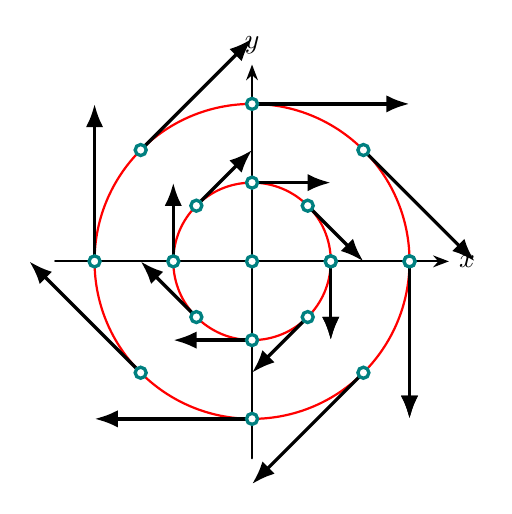
\begin{tikzpicture}[line cap=round, scale = 1]

    \draw[thick, -{Stealth[length=2mm]}] (-2.5, 0) -- (2.5, 0) node[right] {$x$};
    \draw[thick, -{Stealth[length=2mm]}] (0, -2.5) -- (0, 2.5) node[above] {$y$};;
    \draw[fill=none, red, thick](0,0) circle (1);
    \draw[fill=none, red, thick](0,0) circle (2);
    \draw[teal, fill=white, very thick] (0, 0) circle (0.07);
    \foreach \t in {0, 45, 90, 135, 180, 225, 270, 315, 360} {
        \foreach \r in {1, 2} {
            
            \draw[very thick, -Latex] ({\r*cos(\t)}, {\r*sin(\t)}) -- ({\r*cos(\t) + (\r)*cos(\t - 90)}, {\r*sin(\t) + (\r)*sin(\t - 90)});
            \draw[teal, fill=white, very thick] ({\r*cos(\t)}, {\r*sin(\t)}) circle (0.07);
            
        }
        
    }
    \end{tikzpicture}
\end{document}